\subsection{Model Overview}


\figref{fig:overview} gives a general view of our neural network based joint model. The reason we call it a ``Joint Model'' is that the input of neural network is one whole mention table consisting of several cells to be linked, together with a corresponding candidate entity table. All the mentions in the table will be linked simultaneously. The output of our neural network stands for the score of a pair of $\langle T_M, T_E\rangle $, which indicates the probability of choosing that candidate entity table as final result. Specifically, we learn two different features including cell feature and context feature (detailed in \secref{sec:cell}) from the pair of mention table and candidate entity table. To make different representations from two language space compatible, we utilize a bilingual translation matrix to transform the non-English vector into English vector space (detailed in \secref{sec:translation}). Meanwhile, we learn a third feature called coherence feature (detailed in \secref{sec:coherence}) only from the candidate entity table. We then combine these three features together to calculate the final score, which is convenient for training and prediction in this linking task (detailed in \secref{sec:strategy}). 

\begin{figure*}
	\centering
	%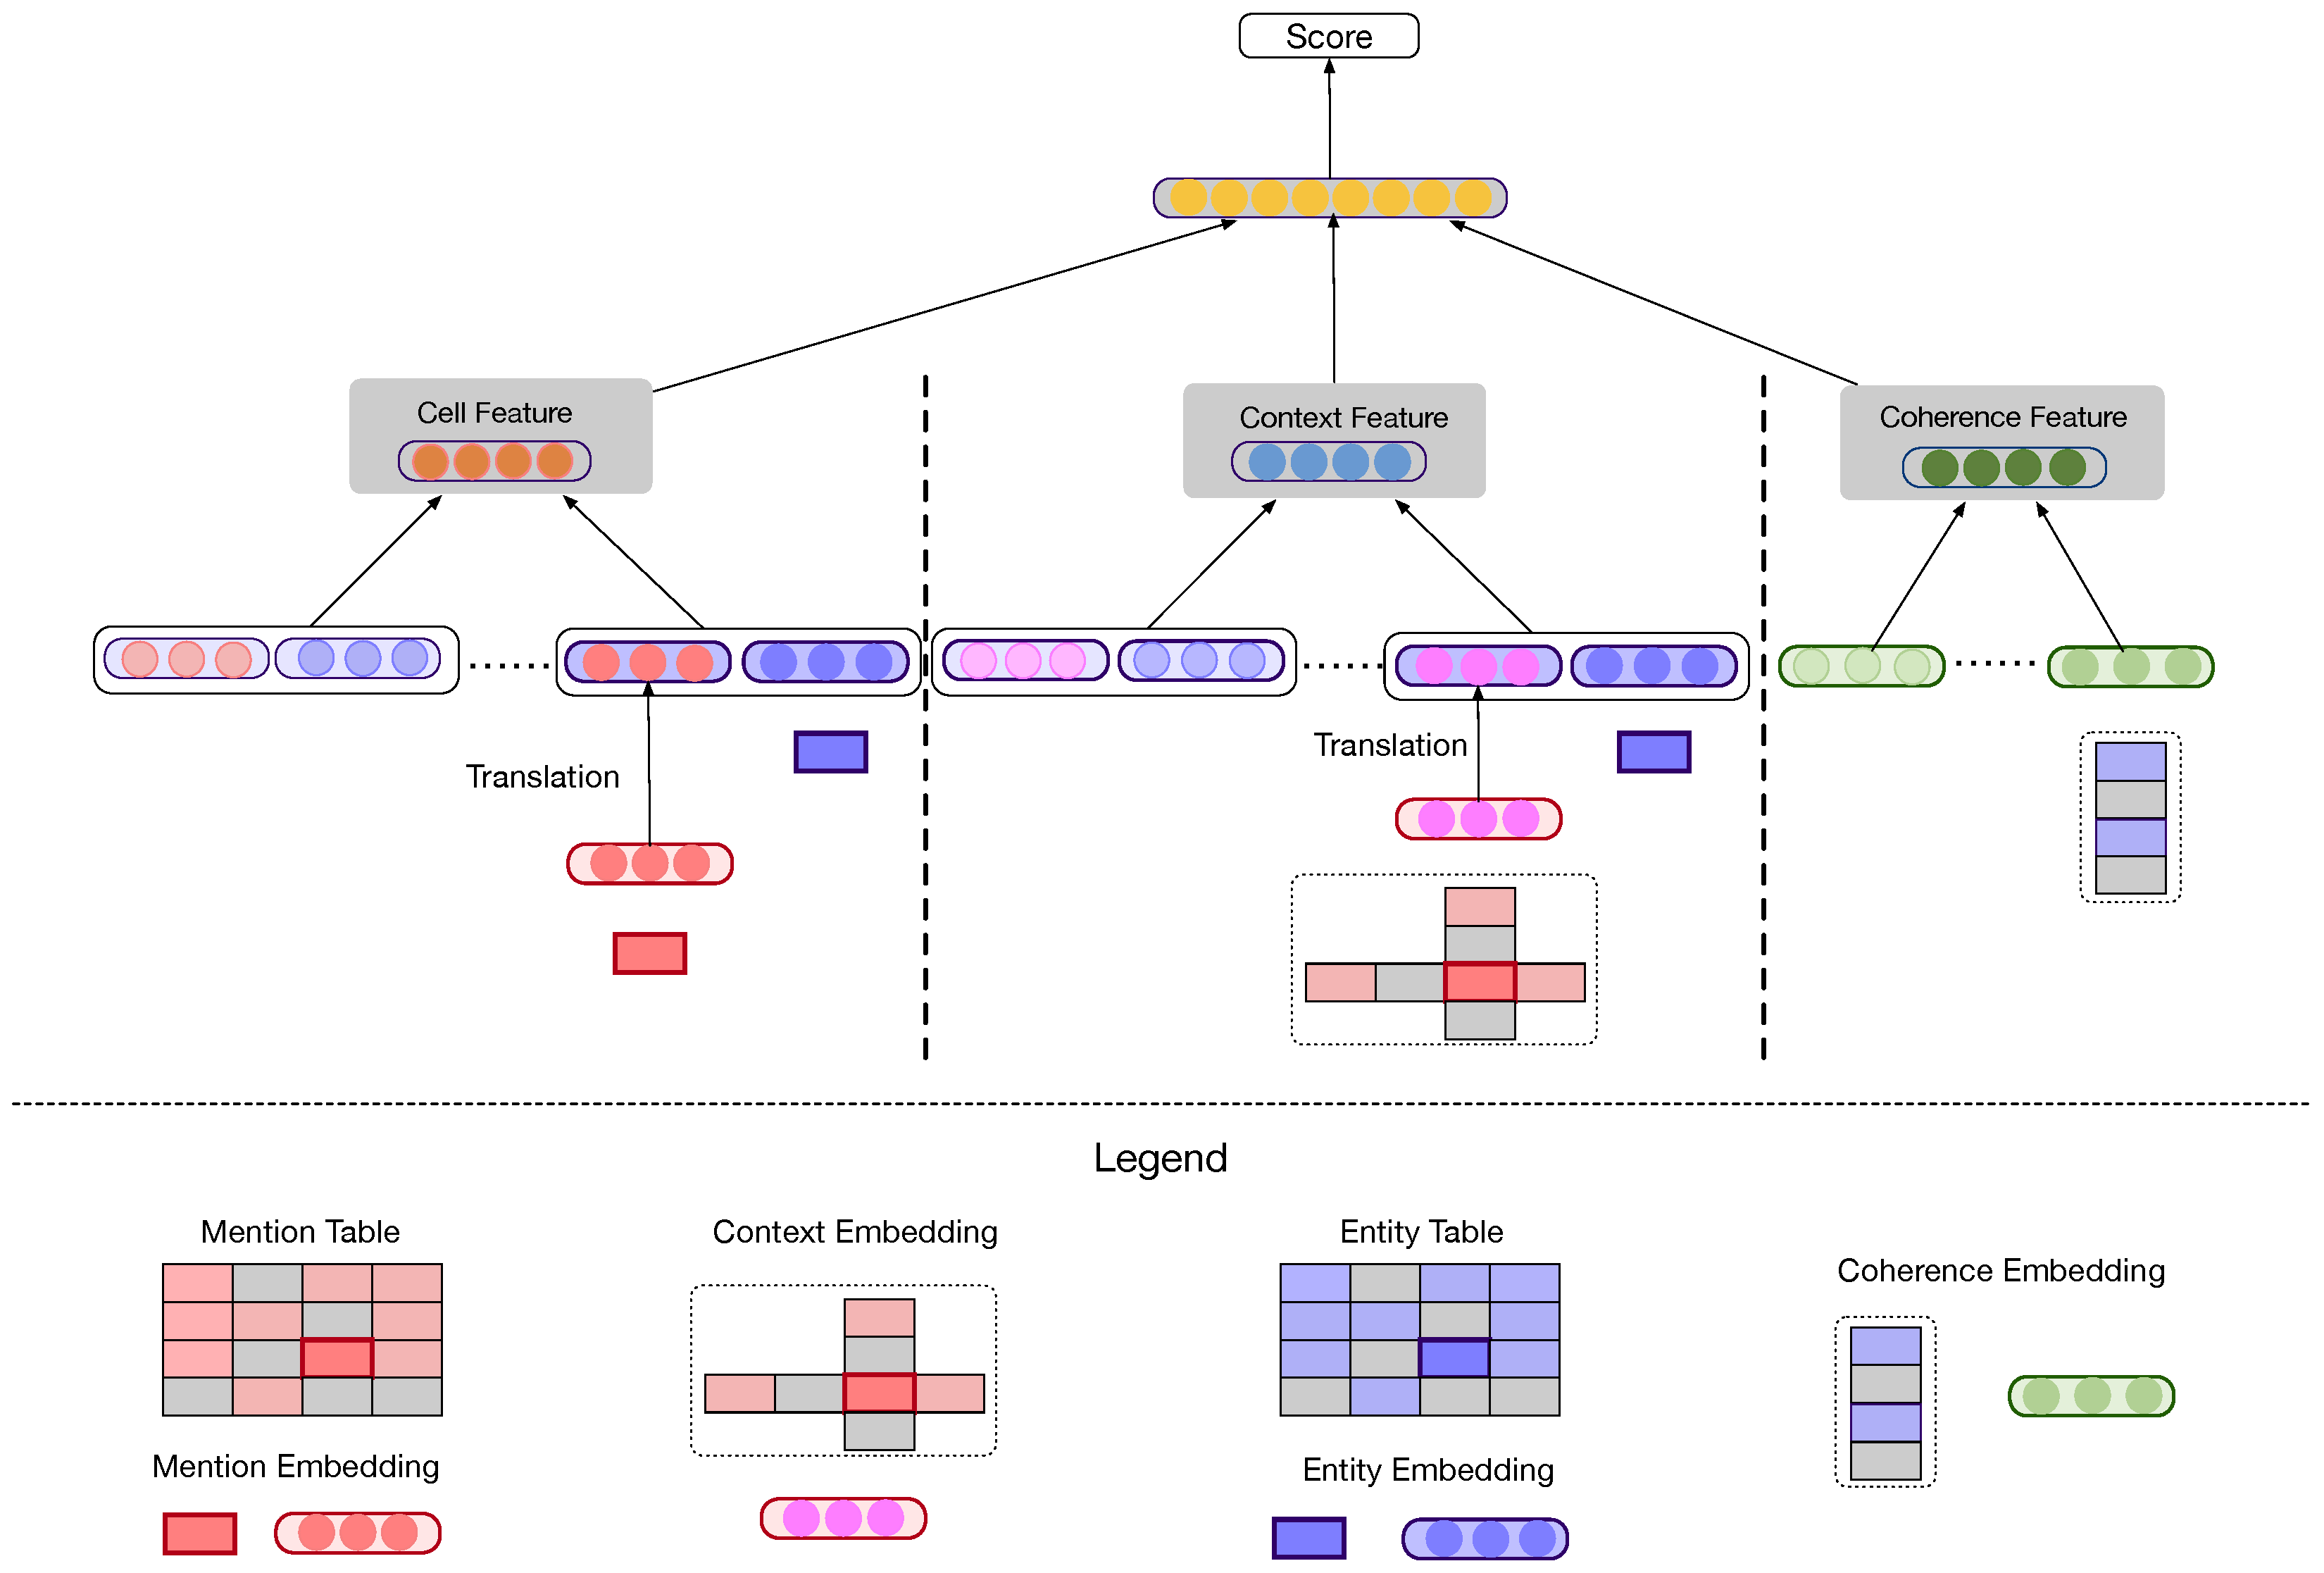
\epsfig{file=overview.eps, angle=0, width=1.0\columnwidth}
	\scalebox{0.3}{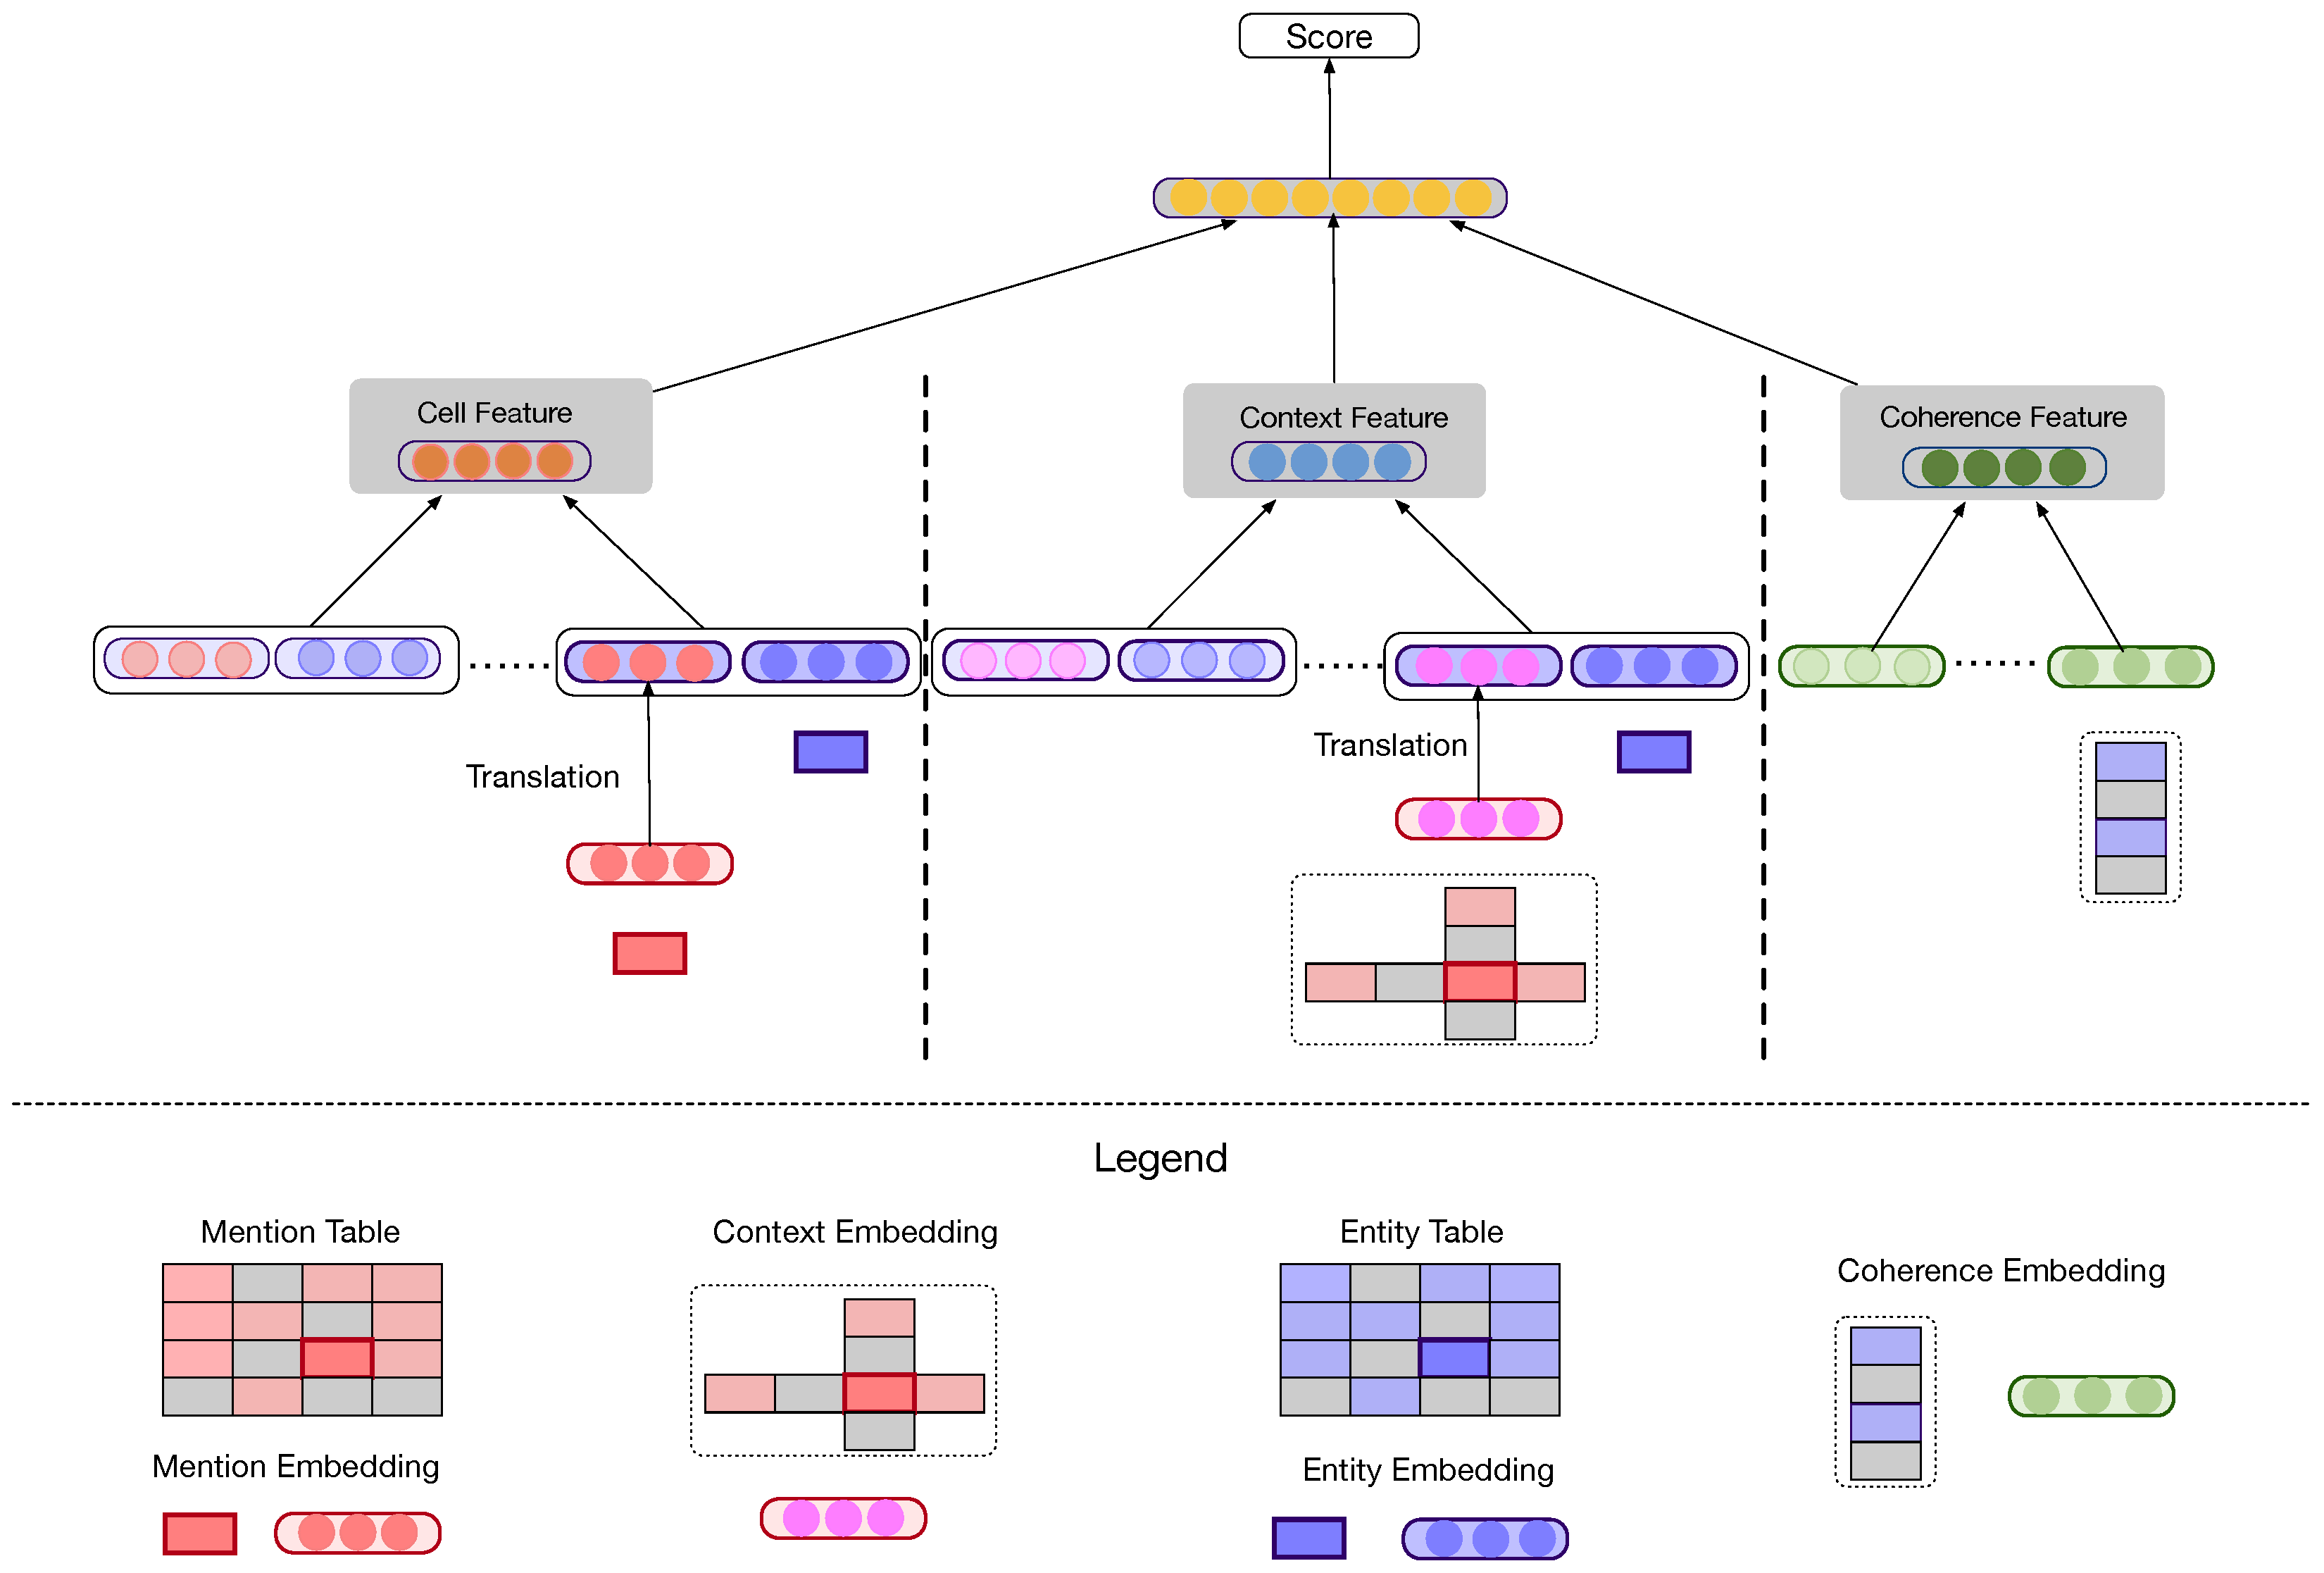
\includegraphics{overview.eps}}
	\caption{Overview of proposed neural network based joint model.}
	\label{fig:overview}
\end{figure*}
